\documentclass[]{article}



\renewcommand{\baselinestretch}{1.2}
\renewcommand{\v}[1]{\ensuremath{\mathbf{#1}}}
\newcommand{\mc}{\mathcal}

\def\st{{\rm s.t.}}

\usepackage{algorithmic}
\usepackage{algorithm}
%\usepackage[usenames,dvipsnames]{color}

\usepackage{todonotes}

\usepackage{fullpage,graphicx,amssymb,amsmath}
\usepackage{enumerate}
\usepackage{subfigure}


\newcommand{\be}{\begin{enumerate}}
\newcommand{\ee}{\end{enumerate}}
\newtheorem{theorem}{Theorem}
\newtheorem{lemma}{Lemma}
\newtheorem{assumption}{Assumption}
\newtheorem{conjecture}{Conjecture}
\newtheorem{corollary}{Corollary}
\newtheorem{definition}{Definition}
\newtheorem{proposition}{Proposition}
\newcommand{\hs}[1]{\hspace{#1}}
\newcommand{\vs}[1]{\vspace{#1}}
\newcommand{\mnorm}[1]{||{#1}||_{\infty}}
\newcommand{\pf}{\textbf{Proof} \indent}
\newcommand{\qed}{\hfill $\Box$}
\newcommand{\argmin}{\rm argmin}
\newcommand{\proof}{\pf}

\newcommand{\Cvar}{\mathbb{CVAR}} % Conditional value-at-risk
%\newcommand{\Cvar}{\mathbb{CV}@\mathbb{R}} % Conditional value-at-risk
\newcommand{\Var}{\mathbb{VAR}} % Value-at-risk
%\newcommand{\Var}{\mathbb{V}\text{a}\mathbb{R}} % Value-at-risk
%\newcommand{\Var}{\mathbb{V}@\mathbb{R}} % Value-at-risk


\usepackage{url}
\newcommand{\cone}{{\rm cone}} % Cone
\newcommand{\conv}{{\rm conv}} % Convex hull
\newcommand{\clconv}{{\rm clconv}} % Closed convex hull
\newcommand{\Cov}{{\rm Cov}} % Covariance
\newcommand{\D}{\mathbb{D}} % Distance metric
\newcommand{\E}{\mathbb{E}} % Expectation
\renewcommand{\P}{\mathbb{P}} % Probability
\renewcommand{\Re}{\mathbb{R}} % Real numbers
\renewcommand{\S}{\mathcal{S}} % Set of scenarios
\newcommand{\Z}{\mathbb{Z}} % Integers

\newcommand{\vell}{\boldsymbol{\ell}}
\newcommand{\valpha}{\boldsymbol{\alpha}}
\newcommand{\vbeta}{\boldsymbol{\beta}}
\newcommand{\vgamma}{\boldsymbol{\gamma}}
\newcommand{\vGamma}{\boldsymbol{\Gamma}}
\newcommand{\vdelta}{\boldsymbol{\delta}}
\newcommand{\vlambda}{\boldsymbol{\lambda}}
\newcommand{\vLambda}{\boldsymbol{\Lambda}}
\newcommand{\vxi}{\boldsymbol{\xi}}
\newcommand{\vpi}{\boldsymbol{\pi}}

\newcommand{\xor}{\underline{\vee}}
\newcommand{\Xor}{\underline{\bigvee}}


\title{Adaptive Distance Metric Selection for Supervised Classification}
\author{Krishnan Kumaran and Dimitri J. Papageorgiou \\
{\small Corporate Strategic Research}\\
{\small ExxonMobil Research and Engineering Company}\\
{\small 1545 Route 22 East, Annandale, NJ 08801 USA}\\
{\small dimitri.j.papageorgiou@exxonmobil.com} \\
}

\begin{document}

\maketitle

\section{Introduction and motivation}

Clustering (also known as unsupervised classification) and Classification (commonly understood to be supervised, i.e., based on training data) are common ways of performing data analysis to perform a range of functions like anomaly detection and diagnosis, data segmentation and model development/refinement. Consequently, there is a large body of research on these topics (see for example [1] and references therein for a survey of currently used methods) offering different solutions ranging from K-means, spectral methods and other more complex methods for Clustering, as well as Support Vector Machines, Artificial Neural Networks (ANN), their non-linear Kernel-based variants and others for Classification.

All clustering methods require a similarity/distance metric between data points. While there are typically a few reasonable choices for most data, the results can depend strongly on this choice. The main goal of this project is to extend existing clustering work (e.g., [2,3,4]) to a semi-supervised classification method that is capable of learning the optimal distance/similarity metric directly from training data. The clustering problem can be formulated as an optimization problem (a mixed-integer linear program in its simplest form) that can be hard to solve for realistic data sizes. This approach using an adaptive distance metric has the potential to provide results of better quality than state-of-the-art techniques like Support Vector Machines.  


\section{Problem statement}

Suppose we are given $N$ points $\v{v}_i \in \Re^p$ with class membership $\mc{C}_i$ for $i \in \mc{N} = \{1,\dots,N\}$.
Our goal is to find a distance metric $\D: \Re^p \mapsto \Re$ such that the following conditions hold:
\begin{enumerate}
\item $\D(\v{v}_i,\v{v}_j) = \v{a}^{\top}(\v{v}_i - \v{v}_j) + (\v{v}_i - \v{v}_j)^{\top} \v{B}(\v{v}_i - \v{v}_j) \quad \forall i,j \in \mc{N}$, for some $\v{a} \in \Re^p$ and $\v{B} \in \Re^{p \times p}$ and symmetric
\item $\D(\v{v}_i,\v{v}_j) \geq 0 \quad \forall i,j \in \mc{N}$
\item $\min_{j \in \mc{C}_i} \D(\v{v}_i,\v{v}_j) < \min_{k \notin \mc{C}_i} \D(\v{v}_i,\v{v}_j) \quad \forall i \in \mc{N}$
\end{enumerate}
Note that this is not a true ``distance metric'' since symmetry and the triangle property are not enforced.
The first condition could be extended to include higher order terms.
Let $\vdelta_{ij} = \v{v}_i - \v{v}_j$ for all $i,j \in \mc{N}$.
Finding such a distance metric can be expressed as the following optimization problem:

 

\begin{subequations} \label{model:1}
\begin{alignat}{4}
\max_{\lambda,\v{a},\v{B},\v{d}}~~& \lambda &&  \\
\st~~& \min_{j \in \mc{C}_i} d_{ij} + \lambda \leq \min_{k \notin \mc{C}_i} d_{ik} & & \qquad \forall i \in \mc{N} \label{eq:separation_requirement} \\
    & d_{ij} = \v{a}^{\top}\vdelta_{ij} + \vdelta_{ij}^{\top}\v{B}\vdelta_{ij} && \qquad \forall i,j \in \mc{N} \\
    & d_{ij} \geq 0 && \qquad  \forall i,j \in \mc{N} \\
    & \v{a} \in \Re^p && \\ 
    & \v{B} \in \Re^{p \times p}, \text{symmetric} &&
\end{alignat}
\end{subequations}

Let $\lambda_i = \left[ \min_{k \notin \mc{C}_i} d_{ik} \right] - \left[ \min_{j \in \mc{C}_i} d_{ij} \right]$ be the difference between the separation/distance from point $i$ to its nearest nonneighbor and the separation/distance from point $i$ to its nearest neighbor.  Ideally, we would like $\lambda_i > 0$ for all $i$.  However, this might not be possible when restricted to a set of distance functions.
In formulation \eqref{model:1}, we would like to maximize the minimum separation over all points as can be seen by re-writing constraint \eqref{eq:separation_requirement} as
$$
\lambda \leq \lambda_i \qquad \forall i \in \mc{N}
$$ 
and noting that the objective function is to maximize $\lambda$.


\subsection{Potential loss functions}

Let $L(\vlambda) = L(\lambda_1,\dots,\lambda_n)$ be a loss function based on the separation of each point $i$. 
Let $f = -L$ be the negative loss function.
In formulation \eqref{model:1}, we are interested in maximizing the function 
$$
f(\vlambda) = -L(\vlambda) = \min_{i \in \mc{N}} \lambda_i~.
$$
Of course, other loss functions are possible and should potentially be considered.

Option 1: Assume $f$ is linear and separable: 
\begin{equation}
f(\vlambda) = \sum_{i \in \mc{N}} f_i(\lambda_i)
\end{equation}

Option 2: Assume $f$ is piecewise linear increasing and separable: 
\begin{equation}
f^{\textrm{PWL-Cont}}(\lambda_i) = \left\{
\begin{array}{ll}
\alpha \lambda_i & \lambda_i \geq 0 \\
\beta \lambda_i & o.w. \\
\end{array}
\right.
\textrm{with } \alpha \leq \beta
\end{equation}

Option 3: Assume $f$ is piecewise linear, increasing up to a  and separable: 
\begin{equation}
f^{\textrm{PWL-DisCont}}(\lambda_i) = \left\{
\begin{array}{ll}
\alpha \lambda_i & \lambda_i \geq 0 \\
\beta & o.w. \\
\end{array}
\right.
\textrm{with }
\end{equation}
 

\begin{figure}[htbp]
\begin{center}
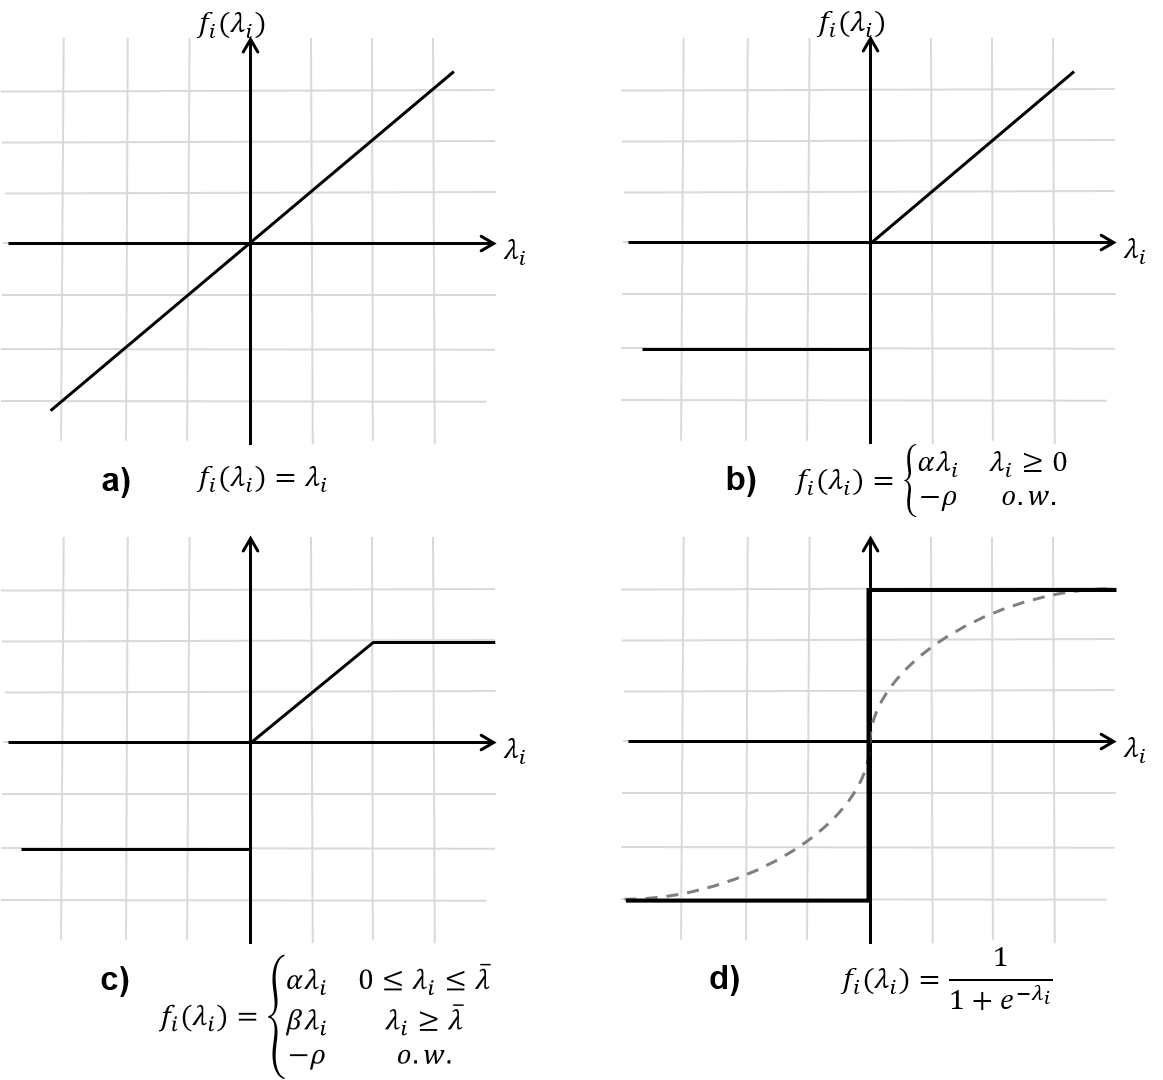
\includegraphics[scale=0.7]{Loss_functions_concatenated.png}
%\vspace{-0.25in}
\caption{Potential loss functions}
\label{fig:loss_functions_concatenated}
\end{center}
\end{figure}


\begin{figure}[htbp]
\begin{center}
%\includegraphics[width=5.0in,height=2.5in]{Circles_before_and_after_basic_step.png}
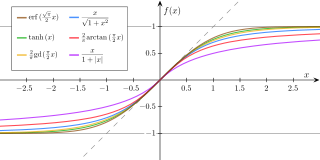
\includegraphics[scale=0.7]{sigmoid_from_wikipedia.png}
%\vspace{-0.25in}
\caption{Sigmoid function. [Source: wikipedia]}
\label{fig:sigmoid}
\end{center}
\end{figure}


\subsection{Imposing a $K>1$ nearest neighbor condition}

Let $d_{i(j)}$ denote the distance of the $j$th closest point to point $i \in \mc{N}$, i.e.,
$d_{i(1)} \leq d_{i(2)} \dots\leq d_{i(|\mc{C}_i|)}$. 
Then, inequality \eqref{eq:separation_requirement} can be rewritten as 
\begin{equation}
d_{i(1)} + \lambda \leq d_{ik} \forall i \in \mc{N}, k \notin \mc{C}_i
\end{equation}

A more restrictive requirement 
\begin{equation}
d_{i(t)} + \lambda \leq d_{ik} \forall i \in \mc{N}, k \notin \mc{C}_i
\end{equation}

The above model can be generalized so that the requirement in inequality \eqref{eq:separation_requirement} holds for the $K$ closest points $j \in \mc{C}_i$, and 






\newpage
%\section{A linear programming approach to a Feasibility Variant of Model \eqref{model:1}}
\section{A linear programming approach to determine the existence of a feasible distance metric}

Let $\mc{F}$ denote the feasible region associated with the distance metric parameters, i.e.,
\begin{equation}
\mc{F} = \{ (\v{a},\v{B},\v{d}) \in \Re^p \times \Re^{p \times p} \times \Re_+^{N \times N} : \v{B}~\text{symmetric}, d_{ij} = \v{a}^{\top}\vdelta_{ij} + \vdelta_{ij}^{\top} \v{B}\vdelta_{ij} \quad \forall i,j \in \mc{N} \}
\end{equation}
or
\begin{subequations} \label{set:feasible_region_distance_metric}
\begin{alignat}{4}
\mc{F} = \Bigg\{ \v{a},\v{B},\v{d} : &  &&  \\
    & d_{ij} = \sum_{k=1}^p \delta_{ijk} a_{k} + \sum_{k=1}^p \delta_{ijk}^2 b_{kk} + 2 \sum_{k=1}^{p-1} \sum_{\ell=k+1}^p  \delta_{ijk} \delta_{ij\ell} b_{k\ell} && \qquad \forall i,j \in \mc{N} \label{eq:distance_metric_def} \\
    & 0 \leq d_{ij} \leq 1 && \qquad \forall i,j \in \mc{N} \\
    & \v{a} \in \Re^p && \\ 
    & b_{k\ell} \in \Re && \qquad \forall k=1,\dots,p, \ell=k,\dots,p \Bigg\}
\end{alignat}
\end{subequations}

The existence of a distance metric satisfying conditions 1-3 can be expressed as the following feasibility (nonlinear optimization) problem, where $\epsilon > 0$ is a given parameter:
%\begin{subequations} \label{model:1_feasibility}
%\begin{alignat}{4}
%\max_{\v{a},\v{B},\v{d}}~~& 0 &&  \\
%\st~~& \min_{j \in \mc{C}_i} d_{ij} + \epsilon \leq \min_{k \notin \mc{C}_i} d_{ik} & & \qquad \forall i \in \mc{N} \label{eq:separation_requirement_eps} \\
%    & d_{ij} = \v{a}^{\top}\vdelta_{ij} + \vdelta_{ij}^{\top} \v{B}\vdelta_{ij} && \qquad \forall i,j \in \mc{N} \\
%    & d_{ij} \geq 0 && \qquad  \forall i,j \in \mc{N} \\
%    & \v{a} \in \Re^p && \\ 
%    & \v{B} \in \Re^{p \times p}, \text{symmetric} &&
%\end{alignat}
%\end{subequations}
\begin{subequations} \label{model:1_feasibility}
\begin{alignat}{4}
\max_{\v{a},\v{B},\v{d}}~~& 0 &&  \\
\st~~& \min_{j \in \mc{C}_i} d_{ij} + \epsilon \leq \min_{k \notin \mc{C}_i} d_{ik} & & \qquad \forall i \in \mc{N} \label{eq:separation_requirement_eps} \\
    & (\v{a},\v{B},\v{d}) \in \mc{F} &&
\end{alignat}
\end{subequations}
Note that if we constrain the distances to be bounded (e.g., $d_{ij} \in [0,1]$), problem \eqref{model:1_feasibility} is not guaranteed to be feasible for an arbitrary choice of $\epsilon$. 
To see this, let $\epsilon > 0$ and consider an example with three points and two classes.  Point 1 is located at (0,0), point 2 at (1,1), and point 3 at $(\epsilon/2,\epsilon/2)$.  Points 1 and 2 belong to class 1, while point 3 belongs to class 2. There is no way to create a distance metric that guarantees that $d_{13} > \epsilon$ and $d_{23} > \epsilon$.

There are several ways to proceed.

\subsection{Multi-Objective approach}
Let $W$ be a positive scalar.  
We could solve the following LP that maximizes both $\epsilon$ and the minimum distance variables $t_i$:
\begin{subequations} \label{model:multi_objective_lp_1}
\begin{alignat}{4}
\max_{\v{a},\v{B},\v{d},\epsilon,\v{t}}~~& W\epsilon + \sum_{i \in \mc{N}} t_i &&  \\
\st~~& t_i + \epsilon \leq d_{ik} && \qquad \forall i \in \mc{N}, k \in \mc{N}\backslash\mc{C}_i \label{eq:mo_lp_separation_constr_t} \\
    & t_i \leq d_{ij} && \qquad \forall i \in \mc{N}, j \in \mc{C}_i \label{eq:mo_lp_dual_constr_t} \\
    & t_i \geq 0 & & \qquad \forall i \in \mc{N} \\
    & \eqref{set:feasible_region_distance_metric} & & 
\end{alignat}
\end{subequations}
\begin{proposition}
Problem \eqref{model:multi_objective_lp_1} is always feasible.
\end{proposition}
\proof The origin is always a feasible solution.  That is, set $\v{a} = \v{0},\v{B} = \v{0},\v{d} = \v{0},\epsilon = 0,\v{t} = \v{0}$.
\qed


\subsection{Iterative LP approach}

First solve the following problem to determine the maximum non-neighbor separation $\epsilon$ that is possible. 
\begin{subequations} \label{model:epsilon_lp_1}
\begin{alignat}{4}
\max_{\v{a},\v{B},\v{d},\epsilon}~~& \epsilon &&  \\
\st~~& \epsilon \leq d_{ik} && \qquad \forall i \in \mc{N}, k \in \mc{N}\backslash\mc{C}_i \label{eq:epsilon_lp_separation_constr_t} \\
    & \eqref{set:feasible_region_distance_metric} & & 
\end{alignat}
\end{subequations}
Let $\epsilon^{\max}$ be the maximum non-neighbor separation, i.e., the optimal value of $\epsilon$ in \eqref{model:epsilon_lp_1}.
 Note that this problem is identical to problem \eqref{model:multi_objective_lp_1} after omitting the $\v{t}$ decision variables.  Hence, it is guaranteed to be feasible.

Given $\epsilon \in (0,\epsilon^{\max}]$, model \eqref{model:1} can be expressed as a linear programming feasibility problem:
\begin{subequations} \label{model:big_lp_1}
\begin{alignat}{4}
\max_{\v{a},\v{B},\v{d},\v{t}}~~& \sum_{i \in \mc{N}} t_i &&  \\
\st~~& t_i + \epsilon \leq d_{ik} && \qquad \forall i \in \mc{N}, k \in \mc{N}\backslash\mc{C}_i \label{eq:big_lp_separation_constr_t} \\
    & t_i \leq d_{ij} && \qquad \forall i \in \mc{N}, j \in \mc{C}_i \label{eq:big_lp_dual_constr_t} \\
    & t_i \geq 0 & & \qquad \forall i \in \mc{N} \\
    & \eqref{set:feasible_region_distance_metric} & & 
\end{alignat}
\end{subequations}
For $\epsilon \in (0,\epsilon^{\max}]$, model \eqref{model:big_lp_1} is always feasible since the origin $\v{0}$ is always feasible.
Note that $t_i$ represents the distance to point $i$'s nearest neighbor since constraints \eqref{eq:big_lp_dual_constr_t} ensure that $t_i \leq \min_{j \in \mc{C}_i} d_{ij}$,
while the objective function encourages $t_i = \min_{j \in \mc{C}_i} d_{ij}$ for all $i$.
Meanwhile, constraints \eqref{eq:big_lp_separation_constr_t} ensure that the separation $[\min_{k \in \mc{N}\backslash\mc{C}_i} d_{ik}] - [\min_{j \in \mc{C}_i} d_{ij}]$ is at least $\epsilon$.
If model \eqref{model:big_lp_1} returns a feasible solution with $t_i^* = \min_{j \in \mc{C}_i} d_{ij}^* > 0$ for all $i \in \mc{N}$, then the distance metric satisfies requirements 1-3.
Otherwise there exists a subset $\mc{O}$ of outlier points such that $0 \leq t_i^* < \min_{j \in \mc{C}_i} d_{ij}^*$ for all $i \in \mc{O}$, which means that no such distance metric guaranteeing a minimum separation exists for the choice of $\epsilon$.


The following algorithm can be used to explore potential distance metrics for different levels of separation.  

\begin{algorithm}
%{\small
\caption{Iterative LP Heuristic}
\label{algo:iterative_LP_heuristic}
\begin{algorithmic}[1]
\STATE Solve model \eqref{model:epsilon_lp_1}. Let $\epsilon^{\max}$ be the optimal objective function value.
\STATE Let $\mc{E} = \{ i / \epsilon^{\max} : i=1,\ldots,I \}$ (e.g., $I=10$)
\FOR{ $\epsilon \in \mc{E}$ }
	\STATE Solve model \eqref{model:big_lp_1}.
	\STATE Store the outliers and distance metric
\ENDFOR
\end{algorithmic}
%}
\end{algorithm}



 

\section{Plot of number of outliers as function $\epsilon$}

\todo[inline]{this should be done before next meeting on 2016-10-27}

\begin{itemize}
\item 
  make a plots a number of outliers as function of epsilon
+ show also the datasets which you have used and so on
\item 
  try different datasets, also generate the two gaussian mixtures
\item   find out how to export figure to EPS from AIMMS
\item  change a copy of {\bf output scatter plot} to use the learnt distance measure
\end{itemize}














\newpage
\section{Mixed-Integer Linear Optimization Approaches}

\subsection{Max-Min Approach: Maximize the minimum separation with outliers}

Model \eqref{model:1} can be expressed as a huge mixed-integer linear programming problem:
\begin{subequations} \label{model:milp_with_outlier_detection}
\begin{alignat}{4}
\max_{\lambda,\v{B},\v{d},\v{w},\v{y}}~~& f(\vlambda) = \sum_{i \in \mc{N}} f_i(\lambda_i) = \sum_{i \in \mc{N}} (\lambda_i - \rho z_i) & & \\
\st~~& \sum_{j \in \mc{C}_i} w_{ij} + \lambda_i \leq d_{ik} + M_i z_i  && \qquad \forall i \in \mc{N}, k \in \mc{N}\backslash\mc{C}_i \\
    & \lambda_i \leq 1 - z_i && \qquad \forall i \in \mc{N} \label{eq:outlier_separation_logic} \\
    & w_{ij} \leq d_{ij} && \qquad \forall i \in \mc{N}, i \in \mc{C}_i \label{eq:mccormick_1} \\
    & w_{ij} \leq y_{ij} && \qquad \forall i \in \mc{N}, i \in \mc{C}_i \label{eq:mccormick_2} \\
    & w_{ij} \geq d_{ij} + y_{ij} - 1 && \qquad \forall i \in \mc{N}, i \in \mc{C}_i \label{eq:mccormick_3} \\
    & \sum_{j \in \mc{C}_i} y_{ij} = 1 && \qquad \forall i \in \mc{N} \\
    & d_{ij} = \sum_{k=1}^p \delta_{ijk}^2 b_{kk} + 2 \sum_{k=1}^{p-1} \sum_{\ell=k+1}^p  \delta_{ijk} \delta_{ij\ell} b_{k\ell} && \qquad \forall i,j \in \mc{N} \label{eq:big_milp_distance_def_constr} \\
    & b_{k\ell} \in \Re && \qquad \forall k=1,\dots,p, \ell=k,\dots,p \\
    & d_{ij} \geq 0 && \qquad \forall i,j \in \mc{N} \\
    & w_{ij} \geq 0 && \qquad \forall i \in \mc{N}, i \in \mc{C}_i \\
    & y_{ij} \in \{0,1\} && \qquad \forall i \in \mc{N}, i \in \mc{C}_i \\
    & z_{i} \in \{0,1\} && \qquad \forall i \in \mc{N} \\
    & \lambda_i \geq 0 & & \qquad \forall i \in \mc{N}
\end{alignat}
\end{subequations}

Model \eqref{model:milp_with_outlier_detection} assumes a linear reward for positive separation and a fixed (constant) penalty $\rho$ for each outlier.  
Outliers are handled through the binary $z_{i}$ decision variables.
If $z_{i} = 1$, then constraint \eqref{eq:outlier_separation_logic} ensures that the separation $\lambda_i$ is 0 and hence ignored; otherwise (if $z_{i} = 0$), this constraint is effectively ignored. 
Constraints \eqref{eq:mccormick_1}-\eqref{eq:mccormick_3} are the so-called McCormick envelopes needed to linearize the bilinear equation $w_{ij} = d_{ij} y_{ij}$.

\todo[inline]{Modify to incorporate assumption that $0 \leq d_{ij} \leq 1$ for all $i$ and $j$.}

 

\subsection{Similar to previous but we will have just one lambda}
\label{sec:mimax_oneLamnda}
\todo[inline]{FInish this soon and compare with previous approach}














\newpage
\section{Generalized disjunctive programming (GDP) formulations}

This section presents several generalized disjunctive programming formulations.

\textbf{Robust GDP formulation with no outliers}
\begin{subequations} \label{model:gdp_robust_no_outliers}
\begin{alignat}{4}
\max_{\lambda,\v{a},\v{B},\v{d}}~~& \lambda &&  \\
\st~~& \mathop{\Xor}_{j \in \mc{C}_i} [ d_{ij} + \lambda \leq d_{ik} \quad \forall k \notin \mc{C}_i ] && \qquad \forall i \in \mc{N} \label{eq:gdp_separation_constr} \\
    & (\v{a},\v{B},\v{d}) \in \mc{F} && 
\end{alignat}
\end{subequations}
Constraints \eqref{eq:gdp_separation_constr} read: ``the distance between point $i$ and its in-class neighbor $j_1 \in \mc{C}_i$ plus the separation $\lambda$ must not exceed the distance between point $i$ and all of its non-neighbors'' or ``the distance between point $i$ and its in-class neighbor $j_2 \in \mc{C}_i$ plus $\lambda$ must not exceed ... '' or ...   

\textbf{Robust GDP formulation with outliers}

\begin{subequations} \label{model:gdp_robust_with_outliers}
\begin{alignat}{4}
\max_{\lambda,\v{a},\v{B},\v{d}}~~& \lambda - \rho \sum_{i \in \mc{N}} z_i &&  \\
\st~~& \Bigg[ \mathop{\Xor}_{j \in \mc{C}_i} [ d_{ij} + \lambda \leq d_{ik} \quad \forall k \notin \mc{C}_i ] \Bigg]~\mathop{\Xor}~[z_i = 1] && \qquad \forall i \in \mc{N} \label{eq:gdp_robust_with_outliers_separation_constr} \\
    & (\v{a},\v{B},\v{d}) \in \mc{F}, \v{z} \in \Re_+^N && 
\end{alignat}
\end{subequations}

\textbf{GDP formulation with outliers}

\begin{subequations} \label{model:gdp_nonrobust_with_outliers}
\begin{alignat}{4}
\max_{\vlambda,\v{a},\v{B},\v{d}}~~& \sum_{i \in \mc{N}} \lambda_i &&  \\
\st~~& \Bigg[ \mathop{\Xor}_{j \in \mc{C}_i} [ d_{ij} + \lambda_i \leq d_{ik} \quad \forall k \notin \mc{C}_i; \lambda_i \geq 0 ] \Bigg]~\mathop{\Xor}~[\lambda_i = -\rho] && \qquad \forall i \in \mc{N} \label{eq:gdp_nonrobust_with_outliers_separation_constr} \\
    & (\v{a},\v{B},\v{d}) \in \mc{F}, \lambda_i \geq -\rho && 
\end{alignat}
\end{subequations}



\newpage
\section{Nomenclature}
\begin{center}
\begin{tabular}{cl}
Decision variable & Definition \\
\hline
$d_{ij}$ & distance between points $i$ and $j$ \\
$w_{ij}$ & $d_{ij}y_{ij}$  \\
$y_{ij}$ & 1 if point $j$ is the closest neighbor to $i$; 0 otherwise  \\
$z_{i}$  & 1 if point $i$ is an outlier; 0 otherwise  \\
$\lambda_i$ & separation (difference) between closest non-neighbor and closest neighbor \\$\lambda_i$ & separation (difference) between closest non-neighbor and closest neighbor \\
$\v{B}$ & $\frac{p(p-1)}{2}$ \\ 
\end{tabular}
\end{center}

\begin{proposition}
Note that we may always assume that the data (input vectors) $v_{i}$ have been normalized to reside in the unit hypercube as follows: $v_{ij} \leftarrow (v_{ij} - m)/(M-m)$ where $m=\min\{v_{ij} : i \in \mc{N}, j=1,\dots,D \}$ and $M=\max\{v_{ij} : i \in \mc{N}, j=1,\dots,D \}$.
\end{proposition}


\newpage
\section{Gershgorin Circle Theorem}

Reference \url{https://en.wikipedia.org/wiki/Gershgorin_circle_theorem}

Why do we care about this theorem? It provides a sufficient condition to ensure that a square matrix is positive semi-definite.

Let $\v{A}$ be a symmetric $n \times n$ matrix (hence, all eigenvalues are real).
Let $R_{i}=\sum _{j\neq {i}} \left|a_{ij}\right|$ be the sum of the absolute values of the non-diagonal entries in the $i$-th row. Let $D(a_{ii},R_{i})$ be the closed circle (or disc) centered at $a_{ii}$ with radius $R_{i}$. Such a disc is called a Gershgorin disc.

\begin{theorem}[Gershgorin Circle Theorem]
Every eigenvalue of $\v{A}$ lies within at least one of the Gershgorin discs $D(a_{ii},R_{i})$.
\end{theorem}

Let $\lambda^{\min}(\v{A})$ be the smallest eigenvalue of $\v{A}$ and let $\lambda_G^{\min}(\v{A}) = \min_{i=1,\ldots,n} \{a_{ii} - R_i\}$.
\begin{corollary}
If $\lambda_G^{\min}(\v{A}) \geq 0$, then $\v{A}$ is positive semi-definite. 
\end{corollary}
\proof Gershgorin's circle theorem asserts that $\lambda_G^{\min}(\v{A})$ is a lower bound on the minimum eigenvalue of $\v{A}$, i.e., $\lambda^{\min}(\v{A}) \geq \lambda_G^{\min}(\v{A})$.  One definition of a psd matrix is that all of its eigenvalues are non-negative. \qed

In our problem, we may require the matrix $\v{B}$ to be positive semi-definite.  Gershgorin's theorem tells us that this can be partially accomplished using linear programming techniques.  (I say ``partially'' because Gershgorin's theorem is not a necessary condition, thus it enforcing $\lambda_G^{\min}(\v{A}) \geq 0$ is actually a restriction, i.e., it may forbid some eligible psd matrices.  Nevertheless, it's an interesting starting point.)  To accomplish this with our matrix $\v{B}$, let $R_{k}(\v{B})=\sum _{\ell \neq k} \left|b_{k\ell}\right|$ and note that the condition $\lambda_G^{\min}(\v{B}) \geq 0$ implies that $\min_{k=1,\ldots,p} \{b_{kk} - R_k(\v{B})\} \geq 0$, which is equivalent to $b_{kk} - \sum _{\ell \neq k} \left|b_{k\ell}\right| \geq 0$ for all $k=1,\ldots,p$.  After introducing auxiliary non-negative decision variables $b^+_{k\ell}$ to model $|b_{k\ell}|$ for all $k \neq \ell$, the latter can be converted into a set of linear constraint as follows:
\begin{subequations} \label{model:gershgorin_restriction}
\begin{alignat}{4}
& b_{kk} - \sum _{\ell \neq k} b^+_{k\ell} \geq 0 && \qquad \forall k=1,\ldots,p \\
& b^+_{k\ell} \geq b_{k\ell} && \qquad \forall k=1,\ldots,p, \ell=1,\ldots,p~(k \neq \ell) \\
& b^+_{k\ell} \geq -b_{k\ell} && \qquad \forall k=1,\ldots,p, \ell=1,\ldots,p~(k \neq \ell) \\
& b^+_{k\ell} \geq 0 && \qquad \forall k=1,\ldots,p, \ell=1,\ldots,p~(k \neq \ell)
\end{alignat}
\end{subequations}

\todo[inline]{In the AIMMS code, we do not store the full $\v{B}$ matrix, but instead work only with the upper diagonal. Thus, it does not make sense to sum over all elements in row $k$ as written in $\sum _{\ell \neq k} b^+_{k\ell}$. Task: Write a similar version of constraints~\ref{model:gershgorin_restriction} in Latex. Implement these additional variables and constraints in AIMMS.  Also, include a binary parameter, say, PI-Require-PSD (use underscores) such that these new variables and constraints are only active if PI-Require-PSD = 1, i.e., you should put a conditional statement ``$|$ ~ PI-Require-PSD'' in the ``index domain'' of these new variables and constraints.
}


\newpage 
\section{Progress Reports 2016-10-21}




\begin{itemize}
\item Loading instance works

\item Solving  \eqref{model:epsilon_lp_1} works now

\item Model \eqref{model:milp_with_outlier_detection}
works. I did it in the aimms code "MILP SECTION4" Part.

\end{itemize}
{\bf problems and questions:}
\begin{itemize}
\item queston 1 How to show the certain points in the plots?
\item question 2

\end{itemize}

{\bf Tasks to do }

\begin{itemize}
\item 1. Create new dataset - e.g.  - Guassian with diffrent mu and Sigma
\item 2. ammend the code to add new point in a.g. Scatter Point
\item 3. Implement Optimization of Distance Metrix                 ACCOMPLISHED
\item 4. Add the robust version for section 4. (have just one lambda) both Latex and AIMS (PROCESSING)
\item 5. Create a performance profiles -- example 100 datasets and comapre 3-4 distance measures 
\item 6. add new codes for replacing "a delta"  - to  "a |delta| "           ACCOMPLISHED
\item 7. add button to load instance          ACCOMPLISHED
\item 8. For Infesible problem we solved during the meeting why it was not infeasible                  ACCOMPLISHED

\end{itemize}

\newpage
\section{Progress Reports 2016-11-04}




\begin{itemize}
\item 1. Create new dataset - e.g.  - Guassian with diffrent mu and Sigma (ACCOMPLISHED)

\item 2. Add the robust version for section 4. (have just one lambda) in AIMMS (ACCOMPLISHED)

\item 3. Find out how to export figure to EPS from AIMMS (PROCESSING)

\item 4. Change a copy of output scatter plot to use the learnt distance measure (ACCOMPLISHED)


\end{itemize}
{\bf problems and questions:}
\begin{itemize}
\item 1. What should I do next? Higher dimension or something else?

\item 2. Still dont know how to draw a circle on a node in AIMMS.

\item 3. I covered the last file u updated by mistake, so I cant see the new theory. Would u please send it to me again? I will merge all of the files in one tex, thx.


\end{itemize}


\newpage
\section{Progress Reports 2016-11-11}

\subsection{Shatter outliers and see $\epsilon$ and Distance Matrices in LP approach}

First run the model in \eqref{model:epsilon_lp_1} in Aimms. 
We do these in Annulus Example 10.1 with 150 points, 2 classes, Probability of outliers = 0.05 and Noise = 0.5.

\begin{figure}[htbp]
\begin{center}
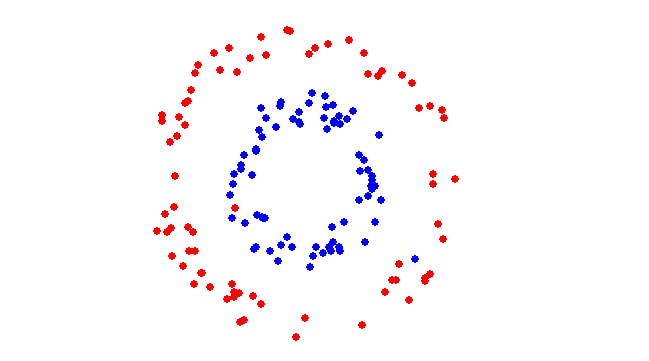
\includegraphics[scale=0.7]{Example_10_1_Origin.PNG}
%\vspace{-0.25in}
\caption{Example 10.1}
\label{fig:Example_10_1_Origin}
\end{center}
\end{figure}

After running the model in \eqref{model:epsilon_lp_1} in Aimms, we get a maximized $\epsilon$ =  0.001113532065 with outliers. 

\begin{figure}[htbp]
\begin{center}
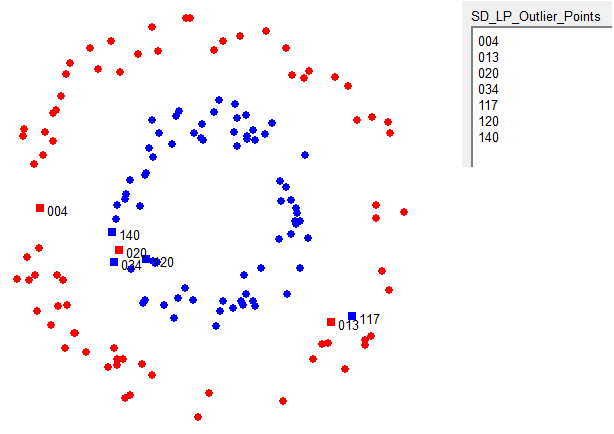
\includegraphics[scale=0.7]{Example_10_1_outliers_1.PNG}
%\vspace{-0.25in}
\caption{Example 10.1 Outliers}
\label{fig:Example_10_1_outliers_1}
\end{center}
\end{figure}

\begin{figure}[htbp]
\begin{center}
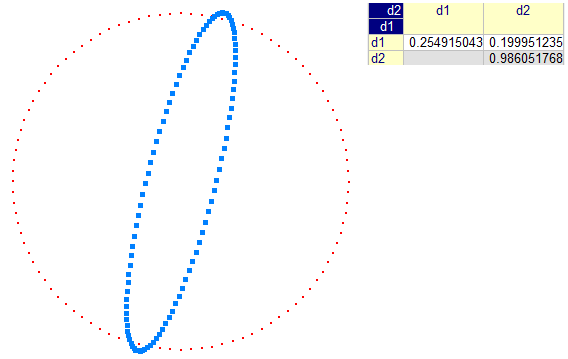
\includegraphics[scale=0.7]{Example_10_1_DistanceMatrix_1.PNG}
%\vspace{-0.25in}
\caption{Example 10.1 DistanceMatrix}
\label{fig:Example_10_1_DistanceMatrix_1}
\end{center}
\end{figure}


\newpage
Now we delete the outliers and do\eqref{model:epsilon_lp_1} in Aimms again. we get a maximized $\epsilon$ =  0.01597093404 with outliers again. This $\epsilon$ is much larger than $\epsilon$ =  0.001113532065 in Example 10.1.

\begin{figure}[htbp]
\begin{center}
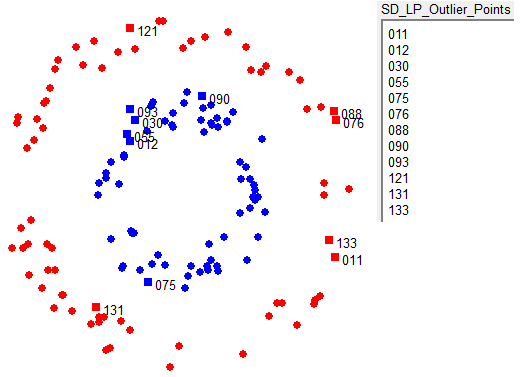
\includegraphics[scale=0.7]{Example_10_2_outliers_1.PNG}
%\vspace{-0.25in}
\caption{Example 10.2 Outliers}
\label{fig:Example_10_2_outliers_1}
\end{center}
\end{figure}

\begin{figure}[htbp]
\begin{center}
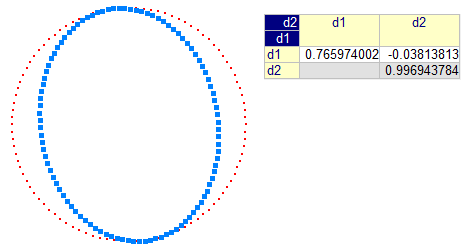
\includegraphics[scale=0.7]{Example_10_2_DistanceMatrix_1.PNG}
%\vspace{-0.25in}
\caption{Example 10.2 DistanceMatrix}
\label{fig:Example_10_2_DistanceMatrix_1}
\end{center}
\end{figure}


\newpage
If we keep running the iterations, we get new outliers with new $\epsilon$ s and different Distance Matrix. In some cases, there will be always outliers after each iteration. Fortunately, In this case, we have only 3 iterations to get no outliers. In iteration 3, $\epsilon$ = 0.01597460757.

\begin{figure}[htbp]
\begin{center}
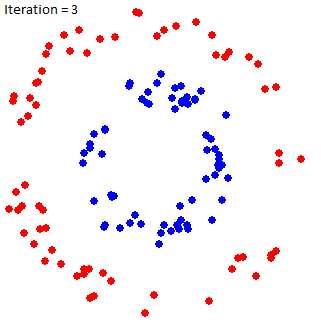
\includegraphics[scale=0.7]{Example_10_3_outliers_1.PNG}
%\vspace{-0.25in}
\caption{Example 10.3 Outliers}
\label{fig:Example_10_3_outliers_1}
\end{center}
\end{figure}

\begin{figure}[htbp]
\begin{center}
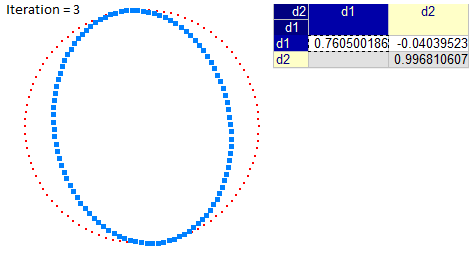
\includegraphics[scale=0.7]{Example_10_3_DistanceMatrix_1.PNG}
%\vspace{-0.25in}
\caption{Example 10.3 DistanceMatrix}
\label{fig:Example_10_3_DistanceMatrix_1}
\end{center}
\end{figure}


\newpage
\subsection{Put back outliers to new model}
We put back outliers to new model to see if they are still outliers.

\begin{figure}[htbp]
\begin{center}
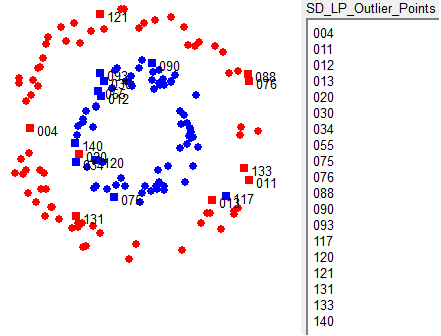
\includegraphics[scale=0.7]{Example_10_3_OutliersBack_1.PNG}
%\vspace{-0.25in}
\caption{Example 10.3 Outliers Back}
\label{fig:Example_10_3_OutliersBack_1}
\end{center}
\end{figure}

Compaired to outliers in previous iterations, the previous outliers are still outliers with new Distance Matrices in iteration = 3.

{\bf problems and questions:}
\begin{itemize}
\item 1. If a case is "unfortunate" one(keeps popping out outliers in each iteration), how do we choose the value of $\epsilon$ to get a solution?

\item 2. I just show some case that "outliers are still outliers",but how do we guarantee others follow the same rule ?

\end{itemize}
\newpage

\section{Progress Reports 2016-11-18}

\begin{itemize}
\item 1. Fix the BUG of mistakes in showing the outliers (ACCOMPLISHED)

\item 2. Fix the mistake of formula using in AIMMS (ACCOMPLISHED)

\item 3. Do Iterations to refill the NonOutliers into the original dataset (Processing)


\end{itemize}
{\bf problems and questions:}
\begin{itemize}
\item 1. AIMMS CODE: How to clone a brand new set from a sub set of "a Set" without any effect when "a Set" changes? Stuck here. 

\end{itemize}


\newpage

\section{Progress Reports 2016-11-21}




\begin{itemize}
\item 1. Deal with all of the Git push and pull problems (ACCOMPLISHED)

\item 2. Do Iterations to refill the NonOutliers into the original dataset (ACCOMPLISHED)

\item 3. The motivation example why we need to remove outliers before learning distance measure (Processing, code done yet no pictures for now)


\end{itemize}
{\bf problems and questions:}
\begin{itemize}
\item 1. 


\end{itemize}

\end{document}



<<<<<<< HEAD
\section{Nomenclature}
=======
\end{document}
>>>>>>> db75255c4a578b567af6b4bab3627c19a3b56451
